\documentclass{article}


% if you need to pass options to natbib, use, e.g.:
%     \PassOptionsToPackage{numbers, compress}{natbib}
% before loading neurips_2022


% ready for submission
% \usepackage{neurips_2022}


% to compile a preprint version, e.g., for submission to arXiv, add add the
% [preprint] option:
\usepackage[preprint]{neurips_2022}


% to compile a camera-ready version, add the [final] option, e.g.:
% \usepackage[final]{neurips_2022}


% to avoid loading the natbib package, add option nonatbib:
%    \usepackage[nonatbib]{neurips_2022}


\usepackage[utf8]{inputenc} % allow utf-8 input
\usepackage[T1]{fontenc}    % use 8-bit T1 fonts
\usepackage{hyperref}       % hyperlinks
\usepackage{url}            % simple URL typesetting
\usepackage{booktabs}       % professional-quality tables
\usepackage{amsfonts}       % blackboard math symbols
\usepackage{nicefrac}       % compact symbols for 1/2, etc.
\usepackage{microtype}      % microtypography
\usepackage{xcolor}         % colors

% my personal packages
\usepackage{tablefootnote}
\usepackage{graphicx}
\bibliographystyle{abbrvnat}


% \title{PPO Agent for LifeSim: a custom Gymnasium Environment based on human daily life simulation}
\title{PPO Agent for LifeSteps: a simulation based on human daily life decisions}


% The \author macro works with any number of authors. There are two commands
% used to separate the names and addresses of multiple authors: \And and \AND.
%
% Using \And between authors leaves it to LaTeX to determine where to break the
% lines. Using \AND forces a line break at that point. So, if LaTeX puts 3 of 4
% authors names on the first line, and the last on the second line, try using
% \AND instead of \And before the third author name.


\author{%
  Daniel Bernardi\\
  MSc Computer Engineering\\
  Alma Mater Studiorum - Bologna\\
  \texttt{daniel.bernardi@studio.unibo.it} \\
  \texttt{daniel\_bernardi@outlook.it}
}


\begin{document}


\maketitle

\begin{abstract}
This paper describes the implementation of a Reinforcement Learning agent using the Proximal Policy Optimization algorithm. The agent interacts with LifeSteps, a customized Gymnasium Environment that simulates various human daily decisions and their impact on life. LifeSteps was developed specifically for this research paper, alongside the algorithm's implementation.
\end{abstract}

\section{Background}

\subsection{Gymnasium}
Gymnasium is an API for Reinforcement Learning that offers a wide range of environments for training and evaluating RL algorithms. It includes support for incorporating new custom environments into the local installation. This feature is valuable because once a custom environment is registered in the local database of environments, it becomes readily usable like any other environment. This guarantees standardized usage and allows for the utilization of wrappers and utilities provided by the Gymnasium library.

\subsection{Proximal Policy Optimization}
The implementation of the Proximal Policy Optimization (PPO) algorithm is a central component of this project, and this section aims to provide background information on it. Since some implementation details of the algorithm can vary, the explanations in this section will provide just enough background for discussing the project's specific implementation. Further informations can be found in the original paper.

PPO builds upon the concepts of Policy Gradient methods and Trust Region methods. 

\textbf{Policy Gradient methods} involve computing the policy gradient, which can serve as input for a stochastic gradient ascent algorithm. Leveraging existing libraries that perform automatic differentiation, this gradient estimator can be obtained by differentiating an objective function using such software.

\textbf{Trust Region Policy Optimization (TRPO)}, introduced by \citet{DBLP:journals/corr/SchulmanLMJA15}), adds a constraint on the size of the policy update. Alternatively, instead of using a constraint, it is possible to incorporate a penalty into the objective function.


PPO implements the idea of a constrained policy update of TRPO in a simple way, based on the following formulas:

\begin{displaymath}
L^{CLIP}(\theta) = \hat{\mathbb{E}}[min(r_t (\theta)\hat{A}_t, clip(r_t(\theta), 1-\epsilon, 1+\epsilon)\hat{A}_t]
\end{displaymath}

With \(r_t(\theta)\) being the ratio between the new and the old policy:
\begin{displaymath}
r_t(\theta) = \frac{\pi_\theta(a_t,s_t)}{\pi_{\theta_{old}}(a_t,s_t)}
\end{displaymath}

And \(\hat{A}_t\) being the advantage function.

The advantage function implemented in PPO is a truncated version of \textbf{Generalized Advantage Estimation} \citep{schulman2018highdimensional}:

\begin{displaymath}
\hat{A}_t = \delta_t + (\gamma\lambda)\delta_{t+1} + \dots + \dots + (\gamma\lambda)^{T-t+1} \delta_{T-1},
\end{displaymath}
\begin{displaymath}
{where\ }\delta_t = r_t + \gamma V(s_{t+1}) - V(s_t)
\end{displaymath}

In conclusion, the objective proposed by PPO is:
\begin{displaymath}
L_t^{CLIP+VF+S}(\theta) = \hat{\mathbb{E}}_t [L_t^{CLIP}(\theta) - c_1 L_t^{VF}(\theta) +c_2S[\pi_\theta](s_t)]
\end{displaymath}

with \(L_t^{VF}(\theta)\) being the mean-squared error loss between the estimated and the target value function, \(S[\pi_\theta](s_t)\) being the entropy of the policy on a given state, and \(c_1\),\(c_2\) two coefficients (hyperparameters).

\paragraph{The algorithm} proceeds with a series of iterations decided by the designer. In each iteration, it collects data by running the policy in the environment and stores (a \textbf{batch} of) the observed states, taken actions, received rewards, and other relevant information. It computes advantages and returns using the collected data. The policy is then updated by optimizing a surrogate objective function. This process is repeated for multiple epochs at each iteration to refine the policy.

This was a summarized review of how PPO works. A more detailed description of the algorithm can be found on the original paper. What has been written here will be basis for discussion in section \ref{trainingloop}.

\section{LifeSteps}
LifeSteps is a single-player game where the player, or an agent, must make decisions on each timestep. Each action taken by the player has consequences that affect their overall progress in the game, requiring strategic thinking to avoid losing. The objective of the game is to keep the player alive until the end of the simulation, which goes on for a fixed number of timesteps. 

LifeSteps offers two game modes: a simple \textit{standard} mode and a more challenging mode called \textit{monopoly}.

\subsection{The standard gamemode}
Since the \textit{monopoly} gamemode is an extension of the \textit{standard}, all of the details written here will be true also for the next section.

The \textbf{life} of the player is the main information contained in every environment's observation. It's implemented as an array of three integers in the interval \([0, 100)\). Each of these integers encode the quality of a part of the player's life: it's \textit{financial resources}, it's \textit{health} and it's \textit{social connections}.

There is also another value, called \textbf{friends}, which tells if the player has at least one true friend. This value doesn't have neither good or bad implications in this gamemode, but it will be important in \textit{monopoly} episodes. 

The \textbf{actions} that the player can perform are three: go to work, do some sport, enjoy a social occasion. 

Each action is linked to a part of the state. When performing an action, the corresponding part of life value will receive a bonus. The other two components will decrease in a deterministic way. 

The difficulty of this simulation is on making the right choices to avoid death (\(\Leftrightarrow\) game is lost), which can happen at any time, when money or value reach the value 0. 

For example, doing sports for a timestep will give a 7 points bonus to the health value, but at the same time the money and social values will decrease of respectively 5 and 1 points.

The \textbf{reward is given to the player only at the end of the simulation}, and is calculated using this formula if the player didn't reach the end of the game:
\begin{displaymath}
    reward = {max\ ts} - {current\ ts} - {difficulty}
\end{displaymath}
If the player accomplished to reach the end of the game, but didn't win, the reward is:
\begin{displaymath}
    reward = min(min(life[i]) - difficulty, 1), i=[money, health, sociality]
\end{displaymath}
with \(life[i]\) being the values about money, health and sociality, and \textit{difficulty} being an initialization parameter of the environment. If the player \textbf{wins} the game, which means that all the life's components have a value higher than the difficulty parameter, the \textbf{reward is 1}.

\subsection{The monopoly gamemode}

In the Monopoly game mode of LifeSteps, similar to the popular table game, players may encounter chance cards that can have negative effects on the game's progression. In LifeSteps, these \textbf{chance cards} represent events that can happen with a certain probability \(p\). After each timestep, the probability of encountering a chance card increases, except when a chance card is drawn, in which case the probability is reset to zero. When an event occurs, a \textbf{points deficit} is applied on the player's health or money, complicating the game. 

The possibility of encountering chance cards events is balanced by another game mechanic, which has no effects in the standard mode: the player's \textbf{friends} state. This information is represented by a boolean value, and it can change only in one direction, from False to True, when the \textit{social} development of the player reaches 40 points. This means that if the player reaches, for example, 43 points on social development, it will acquire a friend, which will remain even if the social development score goes below 40. 

Having a friend in this gamemode provides a significant reduction in the penalties imposed by chance cards events. This features adds variety to the game.

The parameters that define the initial settings of the game are detailed in Table~\ref{gm_start}. The difficulty parameter is chosen by the player upon creating the environment, and the starting values of the state are randomly sampled within their specified range. 

Table~\ref{gm_behaviour} provides an overview of the gameplay behavior, indicating how each state's values increment or decrease at each timestep based on the actions chosen. The increment for a given value is \(0\) only if the corrispondent action is not chosen. Additionally, the penalty applied to one of the life statistics ranges from 0 to 4 if the player has a friend, and 10 otherwise.


\begin{table}
  \caption{Gamemodes initial settings}
  \label{gm_start}
  \centering
  \begin{tabular}{lll}
    \toprule
    & Standard     & Monopoly                               \\
    \midrule
    difficulty              & \([0,100)\)   & \([0,100)\)   \\
    money start             & \([25,34)\)   & \([25,34)\)   \\
    health start            & \([25,34)\)   & \([25,34)\)   \\
    social start            & \([25,34)\)   & \([25,34)\)   \\
    friends start           & \(0\)         & \(0\)         \\
    trouble prob. start     &               & \(0.0\)       \\
    trouble deficit         &               & \([0,4],10\)      \\
    \bottomrule
  \end{tabular}
\end{table}

\begin{table}
  \caption{Gamemodes increments/decrements per timestep}
  \label{gm_behaviour}
  \centering
  \begin{tabular}{rcc}
    \toprule
    & Standard     & Monopoly                           \\
    \midrule
    money inc           & \(0,10\)      & \(0,10\)      \\
    health inc          & \(0,10\)      & \(0,10\)      \\
    social inc          & \(0,10\)      & \(0,10\)      \\
    money dec           & \(-5\)        & \(-5\)        \\
    health dec          & \(-3\)        & \(-3\)        \\
    social dec          & \(-1\)        & \(-1\)        \\
    trouble prob. inc   &               & \(0.03\)      \\
    \bottomrule
  \end{tabular}
\end{table}


\subsection{An example of a LifeSteps simulation}

To better describe how the game works, in Figure~\ref{fig:A} there is an example of the first steps of an episode rendered in text mode.

M, H and S are the three life statistics values: money, health, sociality. The F value describes if the player has some friends. The last column tells if some trouble happened during the last step, indicating also how many points were lost. If the player loses pennies, the deficit goes to the money statistic, if the player get's hurt, the deficit goes to its health.

Let's take into consideration the second and third line. The selected action is sociality, so:
\begin{itemize}
    \item the M value decreases of 5 points (\(\Leftrightarrow 0-5)\);
    \item the H value decreases of 3 points (\(\Leftrightarrow 0-3)\);
    \item the S value increases of 9 points (\(\Leftrightarrow 10-1)\);
\end{itemize}
(0,0,10) is the increase on the state for that timestep (since sociality was selected), (-5,-3,-1) is the constant decrease of the state at each timestep.

In addition to that, the S value is now above the threshold value (40), so the player finally acquires a friend.

\begin{figure}
  \centering
  \fbox{\rule[-.5cm]{0cm}{0cm}
        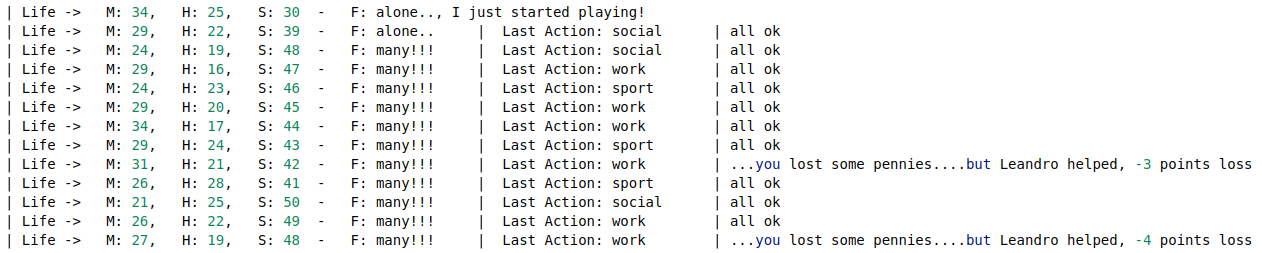
\includegraphics[width=0.95\linewidth]{img/example_A.png}
        \rule[-.5cm]{0cm}{0cm}}
  \caption{The start of an episode in monopoly mode}
  \label{fig:A}
\end{figure}

\section{Implementation}
This section will discuss everything related to the implementation of the algorithm, the architectures of the neural networks, and the structure of the project files and the Jupyter Notebook.

\subsection{Project files}
The project uses entirely the Python language and the code is subdivided in more files to semplify its understanding. The main python files are:

\begin{itemize}
    \item \textit{agent.py}: implements the PPO Agent. Incapsulates the deep learning architecture and all the methods used for training and evaluating the player (works on any gymnasium environment).
    
    \item \textit{memory.py}: creates the memory structures (numpy arrays) that store all the information needed for the calculation of the gradients, the advantages and the returns of each batch.
    
    \item \textit{utils.py}: implements some utility functions, such as the calculation of advantages and returns.
    
    \item \textit{final.ipynb}: the notebook that was executed using seed 14.

    \item \textit{lifesteps.py}: implements the custom gymnasium environment.
\end{itemize}

Since the notebook was executed three times with different seeds, each run was saved into a different file. These files can be found in the \textit{notebook-runs} directory.

The Tensorboard logs of the three runs can be found in the directory \textit{resources/logs/scalars}, and the outputs of the evaluations printed in the notebooks were extracted into txt files inside the \textit{resources/logs/text} directory.

The folder \textit{gym\_projects} contains all the file needed to register the LifeSteps environment into the local Gymnasium installation (the specific environment implementation can be found in \textit{gym\_projects/life\_sim/envs/lifesteps.py}). 

The folder \textit{models} contains the main checkpoints of the deep learning models.

\subsection{Notebook: final.ipynb}
The implementation is done in Python, utilizing the Numpy library for data management and Tensorflow for implementing deep learning models and calculating gradients. The notebook ensures reproducibility at the Numpy and Tensorflow levels. All evaluations are performed on the same environments, initialized with the same seeds. However, it's important to note that the behavior of CUDA is not guaranteed to be deterministic.

The notebook is divided into 4 main Steps:
\begin{itemize}
    \item Step 1: Training and evaluation in the standard game mode with a difficulty level of 40.
    \item Step 2: Fine-tuning and evaluation of the models from the previous step in the monopoly game mode with a difficulty level of 40.
    \item Step 3: Training and evaluation of new models, using the settings from Step 2.
    \item Step 4: Training and evaluation of new models with more units in the hidden layers, using the settings from Step 2.
\end{itemize}

At the beginning of the notebook, a seed is set for the Numpy library, and a collection of seeds is collected. These seeds are used as input for the environments used in the evaluation steps. As a result, even if the seed changes for each run, the 50 evaluation episodes will remain the same.

The notebook has been executed three times, each with a different seed. Each run can be seen in it's specific file called \textit{final-seed\{n\}.ipynb} (in the \textit{notebook-runs} folder) where n represents the seed used for the run. 

The code was executed on a laptop with an Intel® Core™ i7-8565U CPU and an Nvidia MX250 2GB GPU.


\subsection{PPO Actor-Critic}
The Actor-Critic architecture was implemented using two separate neural networks (\(\rightarrow\) no weights sharing) with identical topology, except for the output layers. Each network consists of two hidden dense layer with 32 units each and hyperbolic tangent activations, followed by output heads with linear activations. In Step 4, the number of units was increased to 128 for both models.

The original paper of PPO specifies the design of the algorithm, but many details in implementation can vary: changing the initialization of the neural networks, or the function for calculating the returns and advantages. The notebook follows the fundamental characteristics of the original paper while incorporating some changes.


\subsubsection{The training loop} \label{trainingloop}
Gymnasium provides the possibility to create a vector of multiple environments. This feature was utilized in the notebook by creating an AsyncVec (asynchronous vector) consisting of 32 LifeStep parallel environments. Even if not strictly necessary, this decision accellerated the training process in a considerable way, especially in the monopoly gamemode where many epochs of training were needed to approximate a satisfactory policy.

The algorithm works by optimizing the objective for each \textbf{minibatch}, which is a portion of the total \textbf{batch} of (batch\_length * num\_environments, in this case 128*32) observations. The training loop iterates for a specified number of \textbf{updates}, which depends on the number of parallel environments and the maximum duration of the training (measured in timesteps). For each update, 128 actions are selected for each environment (serialized process w.r.t. the timesteps, parallelized process w.r.t. the environments), forming a batch of \(128 * 32\) sets of informations stored in Numpy NDArrays (observations, rewards, terminations, truncations, state-values). Then, the rewards are normalized and the advantages and returns are calculated for the whole batch.

The batch gets shuffled and subdivided in minibatches, for each of those we perform the optimization step for a specified number of epochs.

Some characteristic of the implementation:
\begin{itemize}
    \item The learning rate and the \(\epsilon\) clipping parameter of PPO are linearly annealed from their starting value to 0 at the end of the training.
    \item Orthogonal initialization of the weights in the neural network.
    \item Reward scaling to the \([-1,1]\) range.
    \item Advantages normalization.
\end{itemize}

The \textbf{advantages} are calculated for all the steps in the batch. The \textbf{returns} are calculated as the discounted sum of the actual rewards, with the exception of the last value, which is calculated using the state-value given by the neural network at the first observation outside the scope of the current batch.

The optimizer used is Adam, same as the original PPO paper. No exhaustive search for the optimal training hyperparameters was performed. The parameters for the PPO algorithm are very similar to the one specified in the original paper.

\subsubsection{Loss function}
PPO is based on gradient ascent, but the popular machine learning frameworks that provides automatic differentiation are based on gradient descent methods. That's why the original PPO objective is changed and minimized for the \textbf{actor network}:

\begin{displaymath}
    Loss_{actor} = -L_t^{CLIP}(\theta) - c_2 S[\pi_\theta](s_t)
\end{displaymath}

The loss minimized on the \textbf{value network} is the mean-squared error between the returns and the approximated state-values.


\section{Results}
Table~\ref{results} summarizes the results of the evaluations for each step and seed, specifying the hyperparameters used. The parameters that were fixed for each training step are listed below:

\begin{itemize}
    \item The max number of timesteps for each episode was 100;
    \item The difficulty level is always 40;
    \item Early stopping of the training was after 6 consecutive evaluations with reward > 0;
    \item \(\gamma = 0.99\) (Discount)
    \item \(\lambda = 0.95\) (GAE parameter)
    \item \(Epochs = 4\)
\end{itemize}

The number of Updates in the table refers to the lenght of the training at the time of the early stopping\footnote{Step 2 is the only one that starts from pre-trained neural networks, so even the number of updates of Step 1 should be considered.}.

\paragraph{A note on the evaluation values}
The values in the Evaluation column are the mathematical mean between the cumulative rewards of 50 episodes. The episodes used for testing the models are the same for every run (even with a different starting seed).
As explained before in section~\ref{trainingloop}, the rewards were scaled into the range [-1,1]. This transformation of the rewards was performed only for the training process, not for the evaluation steps. Since the rewards in LifeSteps are very unbalanced, this must be taken into consideration when discussing the models' performances. 

\begin{table}
  \caption{Training results}
  \label{results}
  \centering
  \begin{tabular}{llcrcccc}
    \toprule
    Model & GM & Units & LR & \(c_2\) & Seed & Updates & Evaluation\\
    \midrule
    Step 1  & std & 32  & 2.5e-4  & 0 & 14 & 350 & \textbf{1.0} \\
    & & & & & 77 & 350 & 0.92 \\
    & & & & & 39 & 350 & 1.0 \\
    \midrule
    Step 2  & mon & 32  & 1e-4   & 5e-3 & 14 & 900 & -1.14\\
    & & & & & 77 & 2343 & -2.04 \\
    & & & & & 39 & 2343 & \textbf{0.66} \\
    \midrule
    Step 3  & mon & 32  & 2.5e-4  & 5e-3 & 14 & 2300 & \textbf{0.72}\\
    & & & & & 77 & 1150 & 0.66 \\
    & & & & & 39 & 3500 & 0.40 \\
    \midrule
    Step 4  & mon & 128 & 2.5e-4  & 5e-4 & 14 & 1750 & \textbf{0.86}\\
    & & & & & 77 & 2300 & 0.86 \\
    & & & & & 39 & 1250 & -0.96 \\
    \midrule
    random-bs  
            & std & & & & 14 & & -122.3 \\
    random-bs
            & mon & & & & 14 & & -126.1 \\
    
    \bottomrule
  \end{tabular}
\end{table}

\section{Discussion}

The PPO Agent solves easily the game in standard gamemode and difficulty 40, with only one lost game between the three runs. 

Step 2 needs some discussion. Its goal was to understand if, starting from pre-trained networks, the training time to play a similar game could be reduced. The results suggest that fine-tuning the neural networks in this particular case does not result in a good evaluation score, most of the time.\footnote{even when fine-tuned models have a decent score, the training time is very long} 

This result isn't that much of a surprise. Since the state is encoded into a 4 values array of integers, the features that the networks need to learn are very simple. 
On the other hand, the policy to win a monopoly episode must be significantly different, and focus on boosting the sociality score from the start to reduce the penalties of chance cards.

Step 3 proves that the monopoly gamemode can be solved, even if the training time is longer than for the standard gamemode. The results are encouraging, the lost games usually where very near to be won by the agent. Another valuable information of this step is that a brand new untrained PPO Agent can perform better, with much less training, than a fine-tuned one taken from Step 2.

There is not a lot to say about Step 4, the results are mainly positive but similar to Step 3, even with the significant increase in hidden layers' units.


\subsection{A deeper analysis}

During each evaluation step, some data about the model's behaviour was collected. To be more specific, it was considered useful to store the overall percentages of chosen actions. The data is described in Table~\ref{behaviour} and the values are taken from the best performer of each gamemode.

This data is not very informative because it's not fine grained, but in a very simple way it describes the overall behaviour of the agent. In the monopoly gamemode, there is need of a more balanced policy for the selection of work and sport actions, to avoid losing the game. Sociality doesn't change much because the difficult is set to 40, which is the threshold to get a new friend. If the difficulty level for the standard gamemode was lower, the sociality actions would decrease. This would't happen with a lower difficult level on monopoly episodes, because the sociality score would still need a boost.

\begin{table}
  \caption{Agent's behaviour during the evaluation steps.}
  \label{behaviour}
  \centering
  \begin{tabular}{lcccc}
    \toprule
    gamemode & seed & work (\%) & sport (\%) & sociality (\%) \\
    \midrule
    standard & 14 & 54.8  & 32.8    & 12.4  \\
    monopoly & 14 & 53.4  & 34.5    & 12.0  \\
    \bottomrule
  \end{tabular}
\end{table}

A standard behaviour for the agent in monopoly mode is to improve the social score during the first timesteps, as seen in Figure~\ref{fig:A}. If this is not accomplished the game would be too hard to beat, as in Figure~\ref{fig:E}. In this example (step 4, seed 39, eval seed 40587), the agent fails to perform enough social actions in the first steps and acquire a friend, which would decrease the health and money losses after chance card events. Since the maximum deficit for a chance card while having a friend is 4, it's easy to see how, with social actions during the two first timesteps, the agent would have lost at least 18 points less. 

\begin{figure}
  \centering
  \fbox{\rule[-.5cm]{0cm}{0cm}
        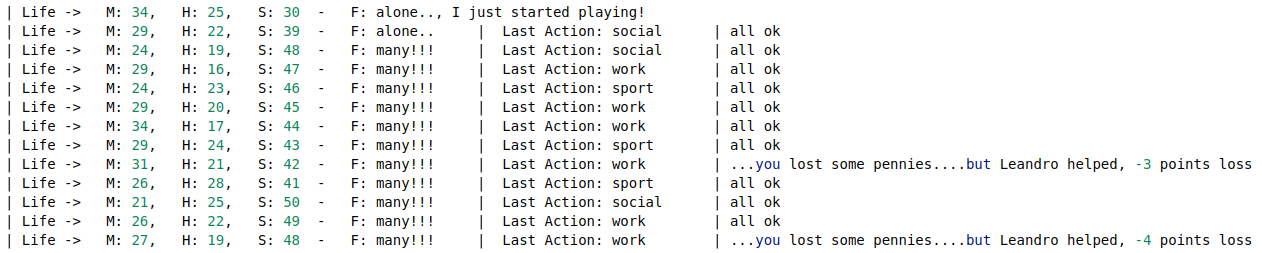
\includegraphics[width=0.95\linewidth]{img/example_A.png}
        \rule[-.5cm]{0cm}{0cm}}
  \caption{The start of an episode in monopoly mode}
  \label{fig:A}
\end{figure}

\begin{figure}
  \centering
  \fbox{\rule[-.5cm]{0cm}{0cm}
        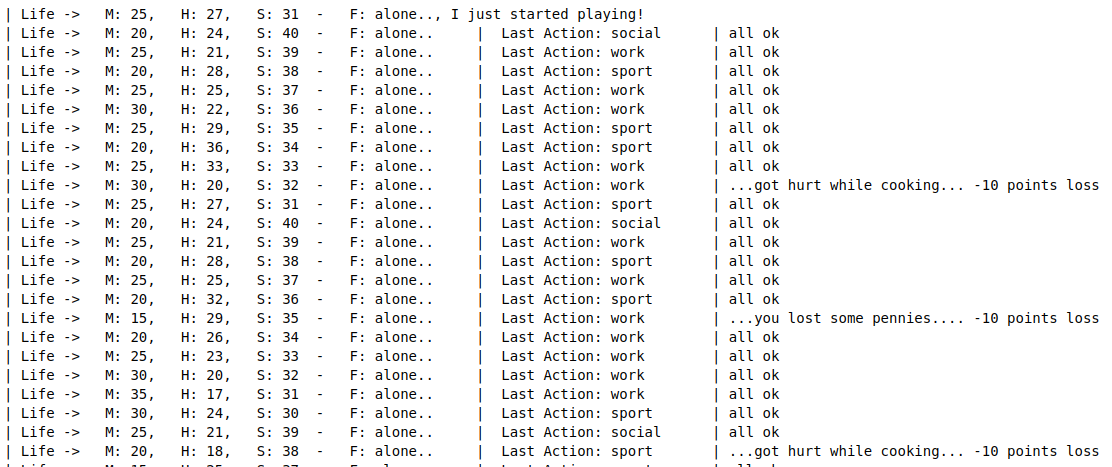
\includegraphics[width=0.95\linewidth]{img/example_E.png}
        \rule[-.5cm]{0cm}{0cm}}
  \caption{A failed monopoly game}
  \label{fig:E}
\end{figure} 

Additionaly, the policy does something strange at the end of a monopoly episode. As can be seen in Figure~\ref{fig:F} (step 4, seed 39, eval seed 75763), the player has a very high social score. The actual social score needed to win the game (in that difficulty level) was 40. On the contrary, the money score is 43, so it seems like the agent takes an unnecessary risk.

\begin{figure}
  \centering
  \fbox{\rule[-.5cm]{0cm}{0cm}
        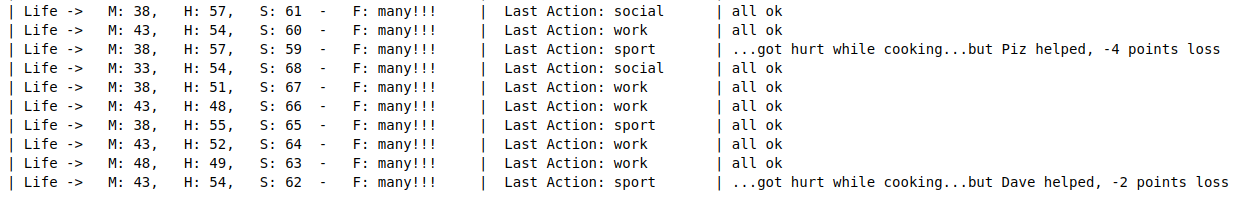
\includegraphics[width=0.95\linewidth]{img/example_F.png}
        \rule[-.5cm]{0cm}{0cm}}
  \caption{Unbalanced life scores at the end of a monopoly episode}
  \label{fig:F}
\end{figure}

A more robust behaviour can be observed at the end of a standard episode, which at the end of the game results in a more balanced life score. 

To understand more the behaviour of the agents it's advisable to read the text logs of the evaluations.

The Tensorboard logs will not be exposed in the report since they don't give out much useful informations. If the reader wants to access them, it can be done opening a local Tensorboard session. The log directory is \textbf{resources/logs/scalars}.

% % % % % % % % % % % % % % % % % % % % % % % % % % % % %
% % % % % % % % % % % % % % % % % % % % % % % % % % % % %
\section{Conclusions}

The LifeSteps environment works correctly and the implemented agent is able to solve the game without many errors. When the game gets difficult, e.g. in monopoly episodes, the agent can still win games but the behaviour seems to be risky and the strategy isn't optimal. Obviously the agents could've been trained more and maybe reach perfect scores even in monopoly gamemode, but that level of performance was not the goal of the project. 

Using vectors of environments proved to be very useful to shorten the length of the training. The agents for the monopoly gamemode would have been very hard to train with a single environment. 

The agent was used (with very little code tweaks) with other environments (e.g. CartPole) to be sure that the algorithm worked well even in different conditions. 

The performance of the trained models seem to be too dependend on the seed. This may be for many reasons such as the randomness and difficulty of the game, or the lack of enough exploration to avoid getting stuck in a local minima. An exhaustive search of optimal hyperparameters (e.g. the entropy bonus) may lead to better performance.


\section{Useful links and references}
\href{https://github.com/ancaah/autonomous}{Project code (github)}

The following arcticles were read to better understand how to implement an effective PPO agent.

\href{https://iclr-blog-track.github.io/2022/03/25/ppo-implementation-details/}{PPO implementation details}

\href{https://github.com/vwxyzjn/cleanrl/blob/master/cleanrl/ppo.py}{CleanRL PPO implementation}

The report was written in english and the phrasing corrected using \href{https://chat.openai.com}{ChatGPT}
%%%%%%%%%%%%%%%%%%%%%%%%%%%%%%%%%%%%%%%%%%%%%%%%%%%%%%%%%%%%

\bibliography{citations}

\end{document}